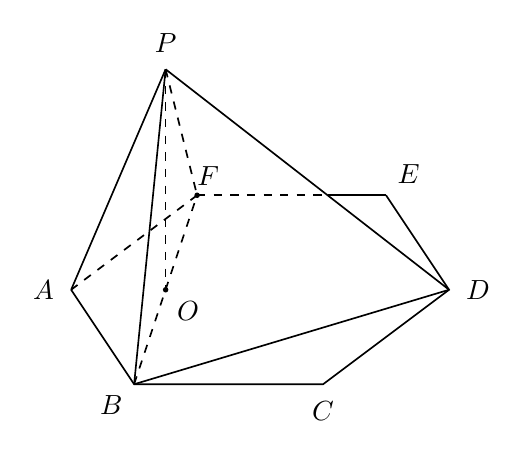
\begin{tikzpicture}[x=1cm,y=1cm,font=\normalsize,
  geometry edge/.style={solid,line width=.6pt},
  geometry label/.style={font=\normalsize,inner sep=2pt}]
% hexagon base ABCDEF (z=0 plane, schematic oblique), O=BF midpoint, P above O
\coordinate (P) at (-1.4,3.6);
\coordinate (A) at (-2.6,0.8);
\coordinate (B) at (-1.8,-0.4);
\coordinate (C) at (0.6,-0.4);
\coordinate (D) at (2.2,0.8);
\coordinate (E) at (1.4,2);
\coordinate (F) at (-1,2);
\coordinate (O) at (-1.4,0.8);
% base outline: front solid, back dashed
\draw[geometry edge] (A)--(B)--(C)--(D)--(E);
\draw[geometry edge,dashed] (F)--(A);\draw[geometry edge,dashed] (F)--(.6571428571,2);\draw[geometry edge] (.6571428571,2)--(E);
% base diagonals
\draw[geometry edge,dashed] (B)--(F);
\draw[geometry edge] (B)--(D);
% apex
\draw[geometry edge] (P)--(A);
\draw[geometry edge] (P)--(B);
\draw[geometry edge] (P)--(D);
\draw[geometry edge,dashed] (P)--(F);
\draw[geometry edge,dashed] (P)--(O);
\fill (O) circle (1pt);
\fill (F) circle (1pt);
% labels offset from strokes
\node[geometry label,above=4pt] at (P) {$P$};
\node[geometry label,left=4pt] at (A) {$A$};
\node[geometry label,below left=2pt] at (B) {$B$};
\node[geometry label,below=4pt] at (C) {$C$};
\node[geometry label,right=4pt] at (D) {$D$};
\node[geometry label,above right=2pt] at (E) {$E$};
\node[geometry label,xshift=4.00bp,yshift=0.00bp] at ([xshift=0pt,yshift=7pt]F) {$F$};
\node[geometry label,below right=2pt] at (O) {$O$};
\end{tikzpicture}
